\section{Adiabatic Quantum Computation}
\label{Section:AQC}
The adiabatic theorem of quantum mechanics provides the foundation for an alternative model of quantum computation based on continuous-time evolution. Consider a time-dependent Hamiltonian $H(t)$ with a discrete and non-degenerate spectrum. Thus we can define its instantaneous eigenstates and eigenenergies by
\begin{equation}
    \hat{H}(t) \ket{n(t)} = E_n (t) \ket{n(t)}.
    \label{eq:instantaneous_eigenstates}
\end{equation}

\noindent As depicted in Fig.~\ref{fig:adiabatic_passage}, the adiabatic theorem states that a quantum system initially prepared in an eigenstate $\ket{n(0)}$ of $H(0)$ will remain in the corresponding instantaneous eigenstate $\ket{n(t)}$ throughout the evolution, provided the spectrum remains gapped and the Hamiltonian changes sufficiently slowly~\cite{sarandy_consistency_2004}. This condition is generally formulated as
\begin{equation}
    T \gg \frac{\mathcal{F}}{\mathcal{G}^2}, 
    \qquad 
    \mathcal{F} = \max_{0 \leq s \leq 1} \big| \bra{k}\,\tfrac{d}{ds}\hat{H}(s)\,\ket{n} \big|, 
    \qquad
    \mathcal{G} = \min_{0 \leq s \leq 1} |g_{nk}(s)| ,
    \label{eq:adiabatic_condition}
\end{equation}
where $T$ is the total runtime, $g_{nk}(s) = E_n(s) - E_k(s)$ is the instantaneous energy gap between levels $n$ and $k$, and $s=t/T$ is the normalized time. In practice, satisfying the adiabatic condition typically requires very long evolution times, which makes implementations vulnerable to decoherence and other noise sources.


\begin{figure}[h]
    \centering
    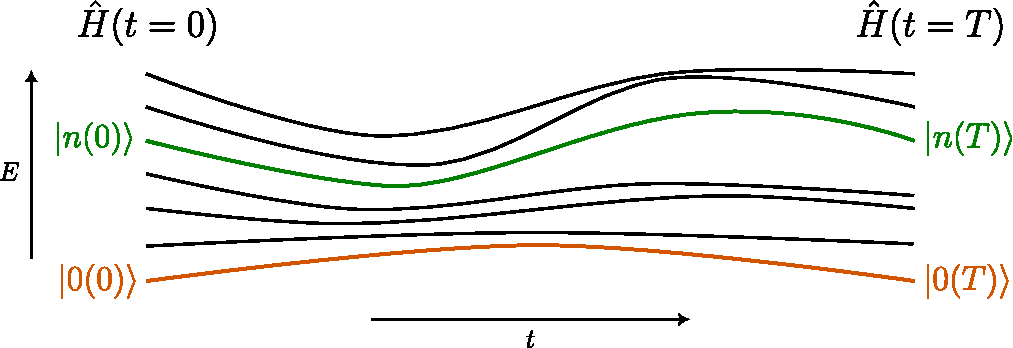
\includegraphics[width=0.75\textwidth]{01-introduction/figs/adiabatic_theorem.pdf}
    \caption{Schematic of an adiabatic passage. The orange line represents the Hamiltonian's ground state, while the green a Hamiltonian's eigenstate different from the ground state.}
    \label{fig:adiabatic_passage}
\end{figure}

Despite the adiabatic theorem works for any eigenstate, in practice it is customary to focus on ground state adiabatic passages. This is because ground states are typically more robust against decoherence and thermal excitations, whenever they are energetically isolated from higher-energy levels. Moreover, for many computational problems, particularly those related to optimization problems, it is possible to construct a Hamiltonian $\hat{H}_\mathrm{P}$ whose ground state encodes the solution to the instance under consideration.

In the adiabatic quantum computation model, the Hamiltonian is interpolated between an initial Hamiltonian $\hat{H}_0$, with a known and easily preparable ground state, and the problem Hamiltonian $\hat{H}_\mathrm{P}$, according to a schedule~\cite{albash_adiabatic_2018}:
\begin{equation}
    \hat{H}(t) = \big[1 - f(t)\big] \hat{H}_0 + f(t) \hat{H}_\mathrm{P}, \quad f(t) \in [0,1],
    \label{eq:adiabatic_passage}
\end{equation}
where $f(t)$ is a smooth, monotonic function such that $f(0)=0$ and $f(T)=1$. The problem Hamiltonian $\hat{H}_\mathrm{P}$ is designed so that its ground state corresponds to the solution of the computational task.

Aharonov et al.~\cite{aharonov_adiabatic_2004} proved that this model is computationally equivalent to the standard circuit model, meaning that any adiabatic process can, in principle, be reproduced digitally with comparable efficiency. This equivalence opens the door to a variety of gate-based approaches that draw inspiration from adiabatic evolution while remaining fully compatible with the circuit model of quantum computation.

\subsection{Adiabatic Quantum Annealers}
An important and widely studied application of adiabatic evolution in quantum devices is Adiabatic Quantum Annealing (AQA), where the goal is to find low-energy configurations of a classical cost function mapped onto a quantum Hamiltonian. AQA is most often applied to Quadratic Unconstrained Binary Optimization (QUBO) problems~\cite{kadowaki_quantum_1998}, which can be exactly reformulated as a 2-body interaction Ising Hamiltonian of the form~\cite{albash_adiabatic_2018}
\begin{equation}
    \hat{H}_\mathrm{P} = \sum_i h_i \hat{\sigma}_i^z + \sum_{i<j} J_{ij} \hat{\sigma}_i^z \hat{\sigma}_j^z\,,
    \label{eq:ising_hamiltonian}
\end{equation}
where $h_i$ are local fields, $J_{ij}$ represent coupling strengths between qubits, and $\hat{\sigma}_i^z$ are Pauli-Z operators acting on the $i$-th qubit, with eigenstates $\ket{0}$ and $\ket{1}$ satisfying $\hat{\sigma}^z \ket{0} = \ket{0}$ and $\hat{\sigma}^z \ket{1} = -\ket{1}$. The task is to drive the system from an initial, easily preparable ground state towards the ground state of $H_\mathrm{P}$, which encodes the optimal solution to the problem at hand.

In a typical AQA protocol, the evolution begins with an initial Hamiltonian of a system with a X-oriented field component of the form
\begin{equation}
    \hat{H}_0 = \sum_i \hat{\sigma}_i^x\,.
    \label{eq:transverse_field_hamiltonian}
\end{equation}
where $\hat{\sigma}^x = \ket{0}\bra{1}+\ket{1}\bra{0}$ and whose ground state is straightforward to prepare. The system is then driven according to the interpolation scheme in Eq.~\eqref{eq:adiabatic_passage}. The aim is to adiabatically steer the system from the easily preparable ground state $H_0$ to the ground state of $H_\mathrm{P}$, which encodes the solution to the problem of interest.

This procedure is feasible for problems that can be expressed in the QUBO form, as they can be mapped to an Ising Hamiltonian with only two-body interactions. This approach has been physically implemented in superconducting-qubit devices, most notably in the commercial quantum annealers developed by D-Wave. However, as we shall see in chapter~\ref{Chapter:Factorization}, the problem of interest in this thesis, integer factorization, does not directly fall into the QUBO class, as its Hamiltonian contains three- and four-body interaction terms.